% !TeX spellcheck = id_ID
\documentclass[a4paper,12pt]{article}
\usepackage[bahasa]{babel}
\usepackage{graphicx}
\usepackage{multirow}
\usepackage{enumitem}
\usepackage[T1]{fontenc}
\usepackage{inconsolata}
\usepackage{lipsum}
\usepackage{xcolor}

\graphicspath{ {./img/} }
\begin{document}
\title{ {\Large Laporan Praktikum}\\ Jaringan Komputer \\{\Large Pertemuan 8}}

\author{Aldzikri Dwijayanto Prathama 
	\\195410189
	\\Teknik Informatika}
\makeatletter
\begin{titlepage}
	\begin{center}
		{\huge \bfseries \@title }\\[14ex]
		
\includegraphics[scale=.8]{logo}\\[4ex]
		{\large \@author}\\[19ex]
		{\large \bfseries {SEKOLAH TINGGI MANAJEMEN INFORMATIKA DAN KOMPUTER
				AKAKOM YOGYAKARTA}}
	\end{center}


%{\large \@date} 
\end{titlepage}
\makeatother
%\maketitle
\newpage
\tableofcontents
\newpage

\section{Tujuan}
Mahasiswa mampu menerapkan routing dinamis dengan RIP pada piranti router

\section{Dasar Teori}
Routing Information Protocol (RIP) adalah sebuah protokol routing dinamis yang digunakan
dalam jaringan LAN (Local Area Network) dan WAN (Wide Area Network). Oleh karena itu protokol ini diklasifikasikan sebagai Interior Gateway
Protocol (IGP). Protokol ini Protokol ini menggunakan algoritma Distance-Vector Routing.
\\
Cara kerja rip:\\

\begin{enumerate}
	\item Host mendengar pada alamat broadcast jika ada update routing dari gateway.
	
	\item Host akan memeriksa terlebih dahulu routing table lokal jika menerima update routing.
	
	\item Jika rute belum ada, informasi segera dimasukkan ke routing table.
	
	\item Jika rute sudah ada, metric yang terkecil akan diambil sebagai acuan.
	
	\item Rute melalui suatu gateway akan dihapus jika tidak ada update dari gateway tersebut dalam waktu tertentu
	
	\item Khusus untuk gateway, RIP akan mengirimkan update routing pada alamat broadcast di setiap network yang terhubung.
	
\end{enumerate}

Karakteristik RIP:\\
\begin{enumerate}
	\item Distance vector routing protocol
	
	\item Hop count sebagi metric untuk memilih rute
	
	\item Maximum hop count 15, hop ke 16 dianggap unreachable
	
	\item Secara default routing update 30 detik sekali
	
	\item RIPv1 (classfull routing protocol) tidak mengirimkan subnet mask pada update
	
	\item RIPv2 (classless routing protocol) mengirimkan subnet mask pada update
	
\end{enumerate}

{\bfseries Kelebihan dan Kekurangan:\\}

\begin{enumerate}
	{\item Kelebihan\\
	RIP menggunakan metode Triggered Update. RIP memiliki timer untuk mengetahui kapan router harus kembali memberikan informasi routing. Jika terjadi perubahan pada
jaringan sementara timer belum habis, router tetap harus mengirimkan ulang informasi routing karena dipicu oleh perubahan tersebut (triggered update).
Mengatur routing menggunakan RIP tidak rumit dan memberikan hasil yang cukup dapat diterima, terlebih jika jarang terjadi kegagalan link jaringan}
	
	{\item Kekurangan\\
	Dalam implementasi RIP memang mudah untuk digunakan, namun RIP mempunyai masalah serius pada Autonomous System yang besar, yaitu:
	\begin{enumerate}[label=\alph*.]
		\item Terbatasnya diameter network, Telah disebutkan sedikit di atas bahwa RIP hanya bisa menerima metrik sampai 15. Lebih dari itu tujuan dianggap tidak terjangkau. Hal ini bisa menjadi masalah pada network yang besar.
		\item Konvergensi yang lambat, untuk menghapus entry tabel routing yang bermasalah, RIP mempunyai metode yang tidak efisien. Seperti pada contoh skema network di atas, misalkan subnet 10 bernilai 1 hop dari router 2 dan bernilai 2 hop dari router 3. Ini pada kondisi bagus, namun apabila router 1 crash, maka subnet 3 akan dihapus dari table routing kepunyaan router 2 sampai batas waktu 180 detik. Sementara itu, router 3 belum mengetahui bahwa subnet 3 tidak terjangkau, ia masih mempunyai table routing yang lama yang menyatakan subnet 3 sejauh 2 hop (yang melalui router 2). Waktu subnet 3 dihapus dari router 2, router 3 memberikan informasi ini kepada router 2 dan router 2 melihat bahwa subnet 3 bisa dijangkau lewat router 3 dengan 3 hop (2 + 1). Karena ini adalah routing baru maka ia akan memasukkannya ke dalam KRT. Berikutnya, router 2 akan meng-update routing table dan memberikannya kepada router 3 bahwa subnet 3 bernilai 3 hop. Router 3 menerima dan menambahkan 1 hop lagi menjadi 4. Lalu tabel routing di-update lagi dan router 2 menerima informasi jalan menuju subnet 3 menjadi 5 hop. Demikian seterusnya sampai nilainya lebih dari 30. Routing akan terus menerus looping sampai nilainya lebih dari 30 hop.
		\item Tidak bisa membedakan network masking lebih dari /24, RIP membaca IP address berdasarkan kepada kelas A, B dan C. Seperti kita ketahui bahwa kelas C mempunyai masking 24 bit. Dan masking ini masih bisa diperpanjang menjadi 25 bit, 26 bit, dan seterusnya. RIP tidak dapat membacanya bila lebih dari 24 bit. Ini adalah masalah besar,
mengingat masking yang lebih dari 24 bit banyak dipakai. Hal ini sudah dapat di atasi pada RIPv2.\\
	\end{enumerate}}
	
\end{enumerate}

Jumlah Host Terbatas\\
\begin{enumerate}
	\item RIP tidak memiliki informasi tentang subnet setiap route.
	
	\item RIP tidak mendukung Variable Length Subnet Masking (VLSM), ketika pertama kali dijalankan hanya mengetahui cara routing ke dirinya sendiri (informasi lokal) dan tidak mengetahui topologi jaringan tempatnya berada
\\
	
\end{enumerate}

Versi\\
Ada tiga versi dari Routing Information Protocol: RIPv1, RIPv2, dan RIPng.
\begin{enumerate}
	\item RIP versi 1\\
	Spesifikasi asli RIP, didefinisikan dalam RFC 1058, routing dengan classfull addressing. Update routing periodik tidak membawa informasi subnet, sehingga tidak mungkin untuk menggunakan metode Variable Length Subnet Mask (VLSM). Keterbatasan ini tidak memungkinkan untuk memiliki subnet berukuran berbeda dalam kelas jaringan yang sama. Dengan kata lain, semua subnet dalam kelas jaringan harus memiliki ukuran yang sesuai dengan kelas IP masing-masing. Selain itu, tidak adanya dukungan untuk router otentikasi, membuat RIP rentan terhadap berbagai serangan.
	\item RIP versi 2
\\
	Karena kekurangan RIP versi 1, RIP versi 2 (RIPv2) dikembangkan pada tahun 1993 dan standar terakhir pada tahun 1998. Ini termasuk kemampuan untuk membawa informasi subnet, sehingga mendukung Classless Inter-Domain Routing (CIDR). Untuk menjaga kompatibilitas, maka batas hop (router) tetap sebanyak 15 hop.
	\item RIPng\\
	RIPng (RIP Next Generation / RIP generasi berikutnya), yang didefinisikan dalam RFC 2080, adalah perluasan dari RIPv2 untuk mendukung IPv6, generasi Internet Protocol berikutnya. Perbedaan utama antara RIPv2 dan RIPng adalah:
	\begin{enumerate}[label=\alph*.]
		\item Dukungan dari jaringan IPv6.
		
		\item RIPv2 mendukung otentikasi RIPv1, sedangkan RIPng tidak. IPv6 router itu, pada saat itu, seharusnya menggunakan IP Security (IPsec) untuk otentikasi.
		
		\item RIPv2 memungkinkan pemberian beragam tag untuk rute, sedangkan RIPng tidak;
		
		\item RIPv2 meng-encode hop berikutnya (next-hop) ke setiap entry route, RIPng membutuhkan penyandian (encoding) tertentu dari hop berikutnya untuk satu set entry route.
		
	\end{enumerate}
	Batasan
	\begin{enumerate}[label=\arabic*.]
		\item Hop count tidak dapat melebihi 15, dalam kasus jika melebihi akan dianggap tidak sah. Hop-tak-hingga direpresentasikan dengan angka 16.
		
		\item Sebagian besar jaringan RIP datar. Tidak ada konsep wilayah atau batas-batas dalam jaringan RIP.
		
		\item Variabel Length Subnet Masks tidak didukung oleh RIP IPv4 versi 1 (RIPv1).
		
		\item RIP memiliki konvergensi lambat dan menghitung sampai tak terhingga bermasalah.
		
	\end{enumerate}
\end{enumerate}

\newpage

\section{Praktik}
\begin{enumerate}
	\item {\bfseries Menghapus konfigurasi Mikrotik
}
	\begin{center}
	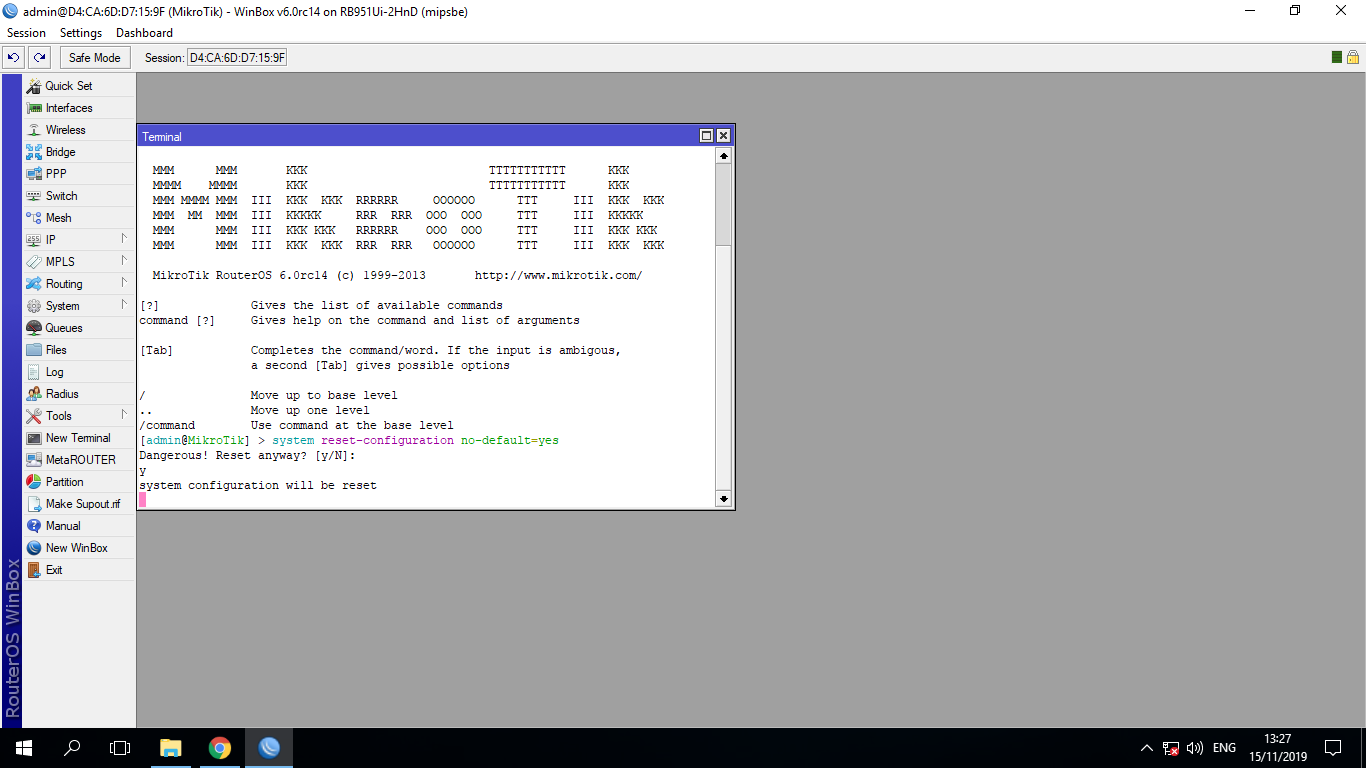
\includegraphics[scale=.4]{Page-1-Image-1}
	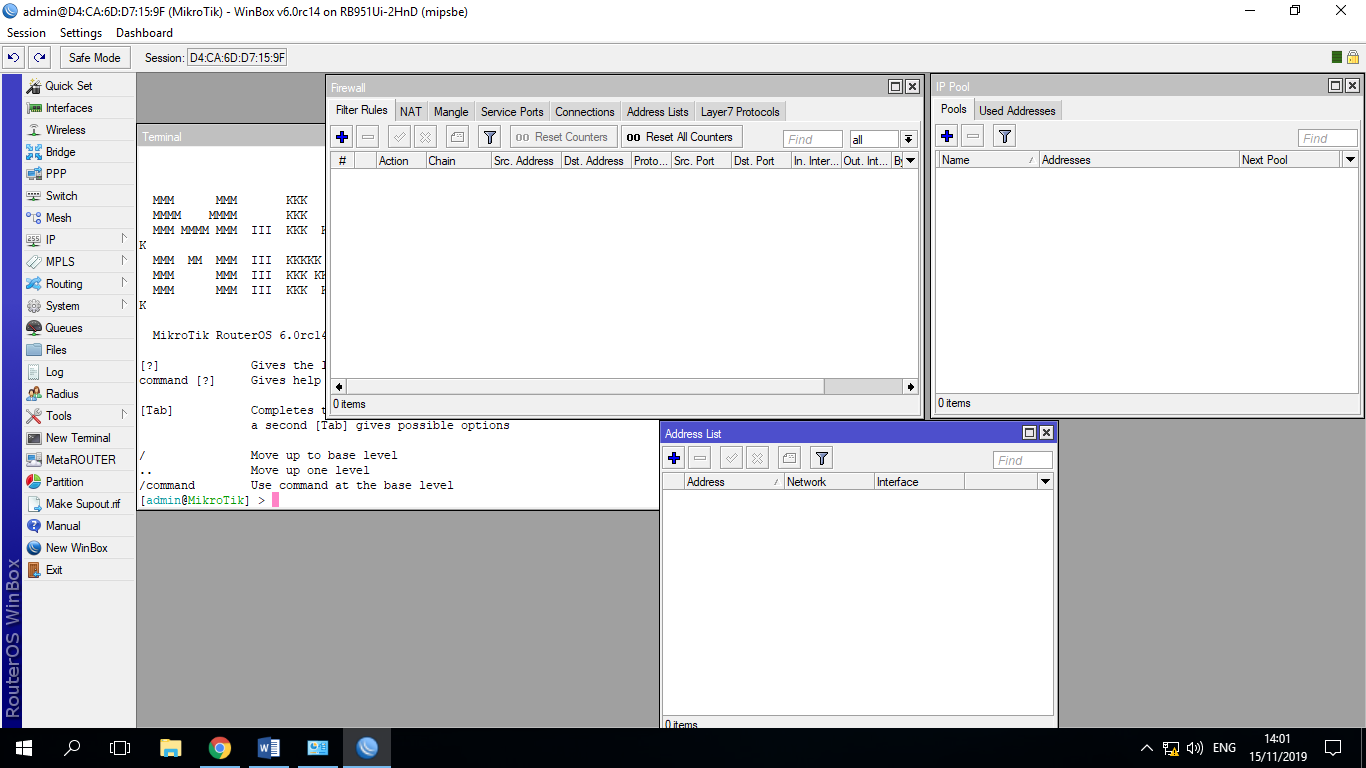
\includegraphics[scale=.4]{Page-1-Image-2}
	\end{center}	
	\begin{enumerate}[label=\alph*.]
		\item Login ke Mikrotik menggunakan WinBox.
		
		\item Klik menu New Terminal
		
		\item Pada prompt command line berikan perintah:
		
		\texttt{>system reset-configuration no-default=yes}
		
		\item Perintah ini menghapus semua konfigurasi router dan menetapkannya ke default untuk nama login dan kata sandi ('admin' dan tidak ada kata sandi), alamat IP dan konfigurasi lainnya akan dihapus, dan antarmuka akan menjadi dinonaktifkan.
		
		\item Tekan Enter, maka akan muncul pertanyaan, untuk konfirmasi apakah akan dilakukan Reset, masukkan y(yes), maka Mikrotik akan booting dan konfigurasinya telah dihapus semua.
		
		\item Masuk kembali ke Mikrotik lewat ether2, menggunakan Mac Address.
		
	\end{enumerate}
	
	\item {\bfseries Instalasi Jaringan\\}
	\begin{itemize}
		\item Pasang 2 Router R951Ui-2HND,
		
		\item 3 kabel  straight UTP
		
		\item Hubungkan ether1 Router 1, ke ether1 Router2
		
		\item Hubungkan masing-masing ethernet2 ke jaringan lokal atau ke PC, seperti pada gambar berikut:
		
	\end{itemize}

	\item \textbf{Menambahkan IP address ether1 dan ether2}
	\begin{center}
		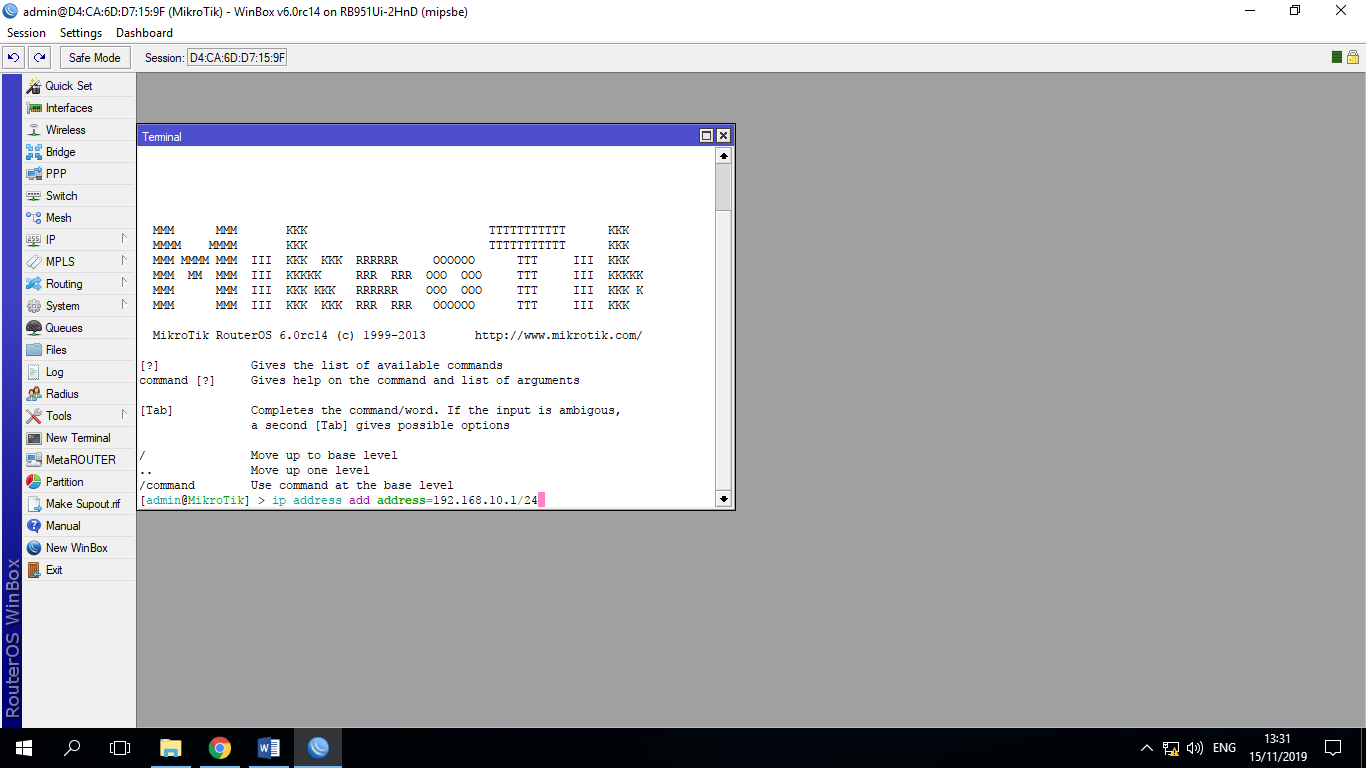
\includegraphics[scale=.4]{Page-2-Image-3}	
	\end{center}
	Pilih new terminal, lalu isikan perintah berikut\\
	\texttt{[admin@MikroTik] >\textcolor{red} {ip address add address=192.168.3.1/24 interface=ether1}}\\
	lalu tekan enter, kemudian masukkan perintah lagi\\
	\texttt{[admin@MikroTik] >\textcolor{red} {ip address add address=192.168.10.1/24 interface=ether2}}\\
	
	\item \textbf{Routing RIP\\}
	\begin{center}
		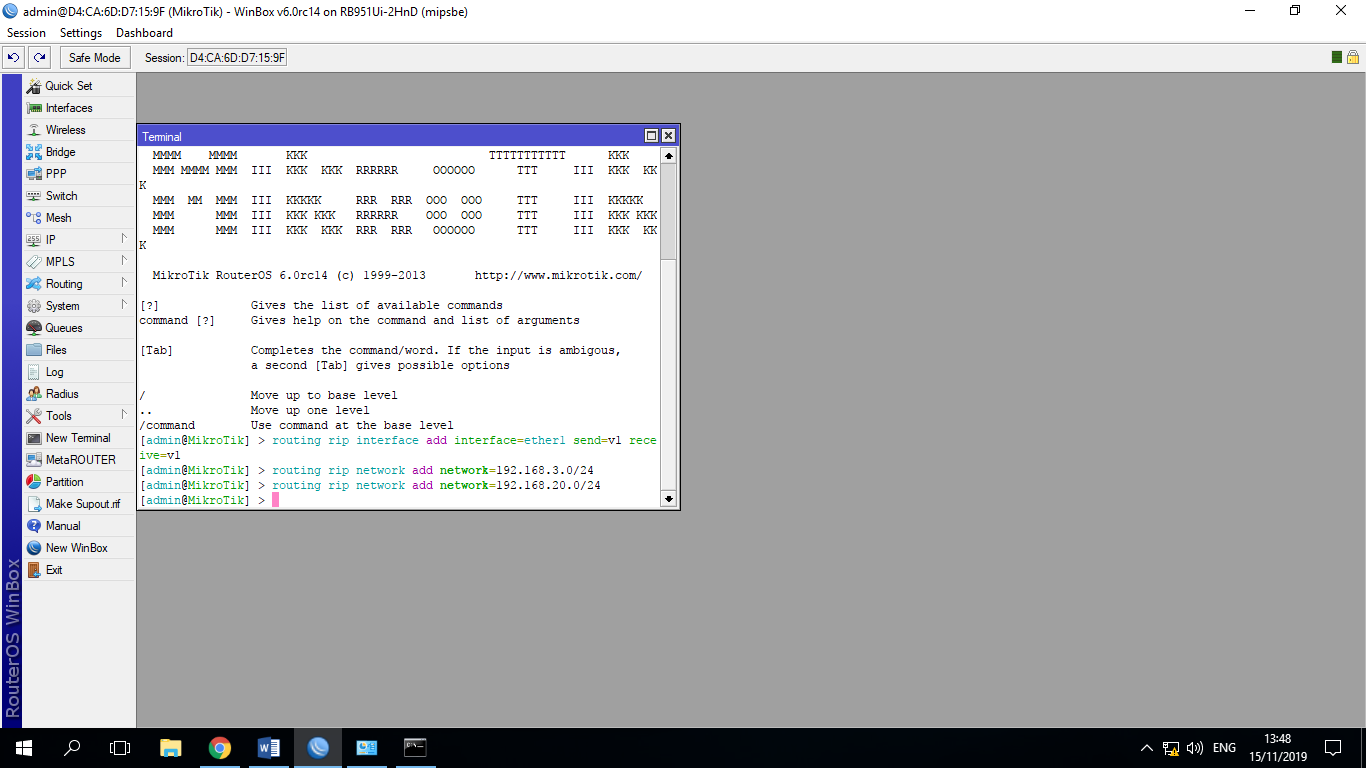
\includegraphics[scale=.4]{Page-3-Image-5}
	\end{center}
	Setelah menambahkan IP ke interface ether1 dan ether2, routing rip dengan perintah\\
	\texttt{[admin@MikroTik] >\textcolor{red}{routing rip interface add interface=ether1 send=v1 receive=v1}}\\
	Tekan enter lalu masukkan perintah\\
	\texttt{[admin@MikroTik] >\textcolor{red}{routing rip network add network=192.168.10.0/24}}\\
	Setelah itu masukkan\\
	\texttt{[admin@MikroTik] >\textcolor{red}{routing rip network add network=192.168.3.0/24}}
	
	\newpage
	
	\item \textbf{Melihat Hasil Routing}
	\begin{center}
		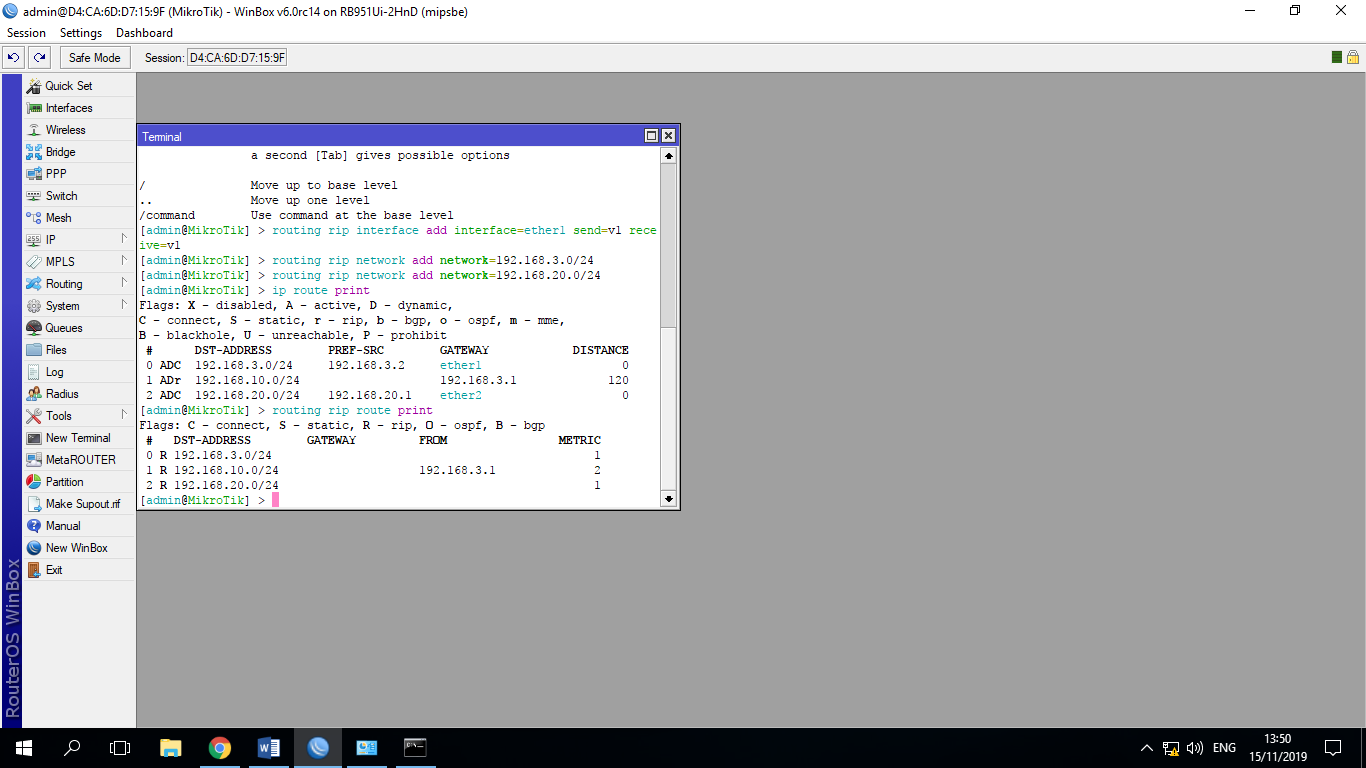
\includegraphics[scale=.4]{Page-3-Image-6}
	\end{center}
	Untuk melihat hasil routing dalam terminal bisa dilakukan dengan perintah:
	\texttt{[admin@MikroTik] > \textcolor{red}{routing rip route print}}
	
	\item \textbf{Menguji koneksi dari PC 2}
	\begin{center}
		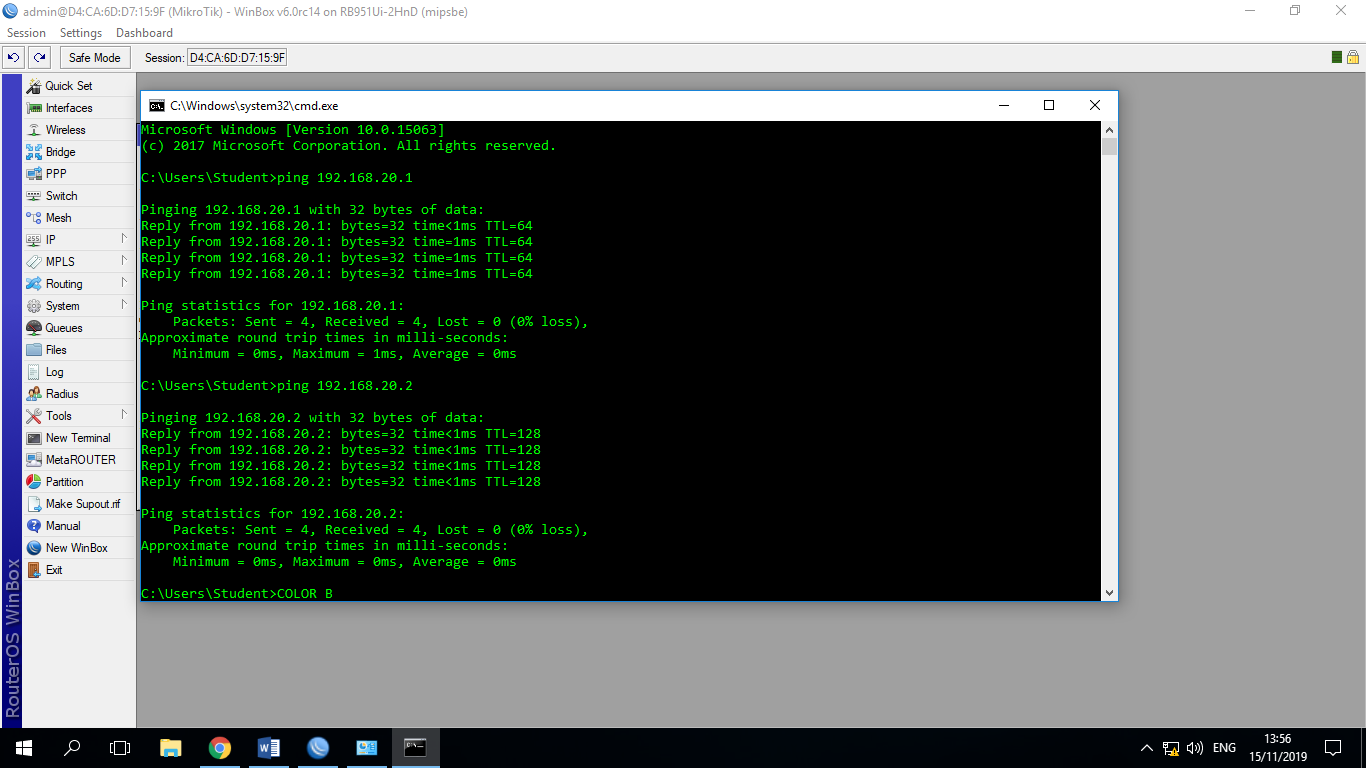
\includegraphics[scale=.38]{Page-4-Image-7}
	\end{center}
	Untuk menguji koneksi kita menggunakan perintah ping
	
	
\end{enumerate}

\section{Latihan}
\paragraph{Konfigurasi RIPv2}
\begin{enumerate}
	\item \textbf{Menambahkan IP address ether1 dan ether2}
	\begin{center}
		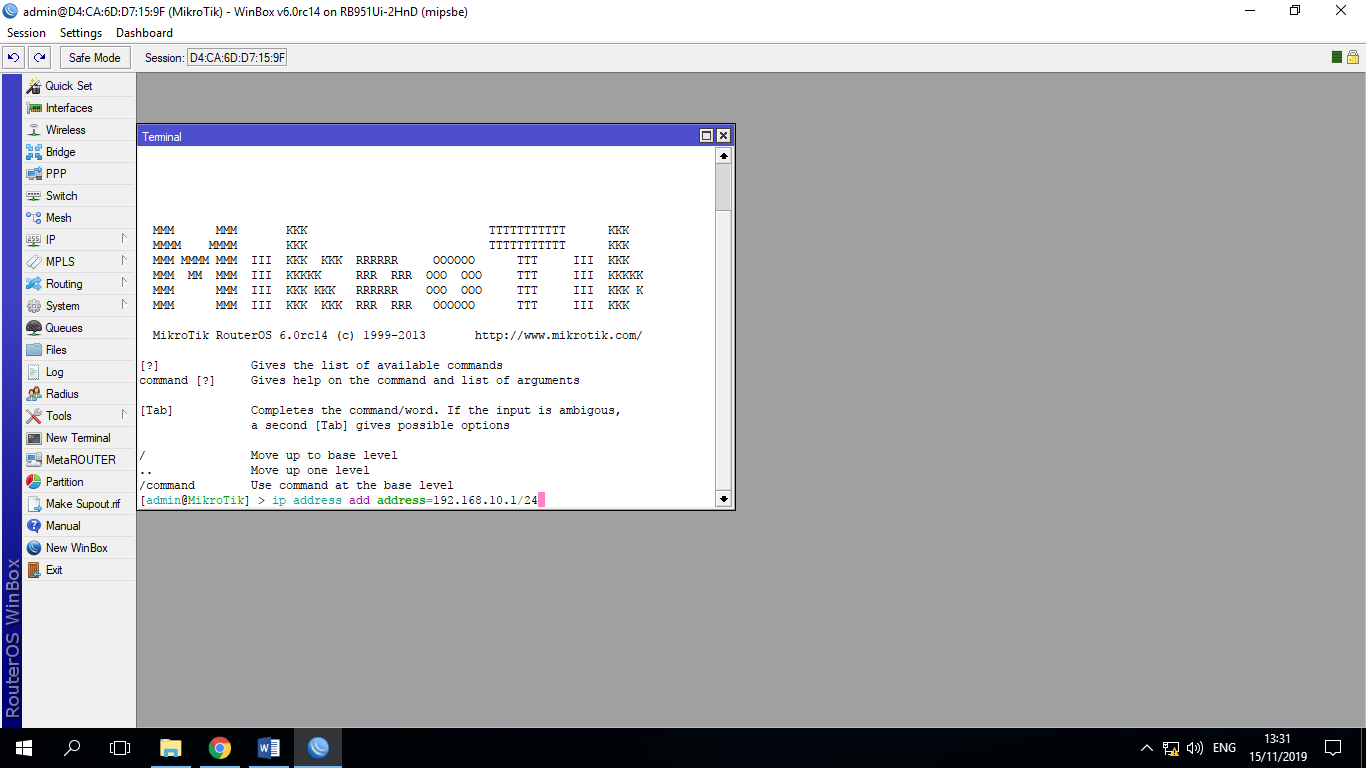
\includegraphics[scale=.38]{Page-4-Image-8}
	\end{center}
	tambahkan ip ke interface eth1 dan ether2 perintah berikut\\
	\texttt{[admin@MikroTik] >\textcolor{red} {ip address add address=192.168.3.1/24 interface=ether1}}\\
	lalu tekan enter, kemudian masukkan perintah lagi\\
	\texttt{[admin@MikroTik] >\textcolor{red} {ip address add address=192.168.10.1/24 interface=ether2}}\\
	
	\newpage
	
	\item \textbf{Setting IP PC 2}\\
	\begin{center}
		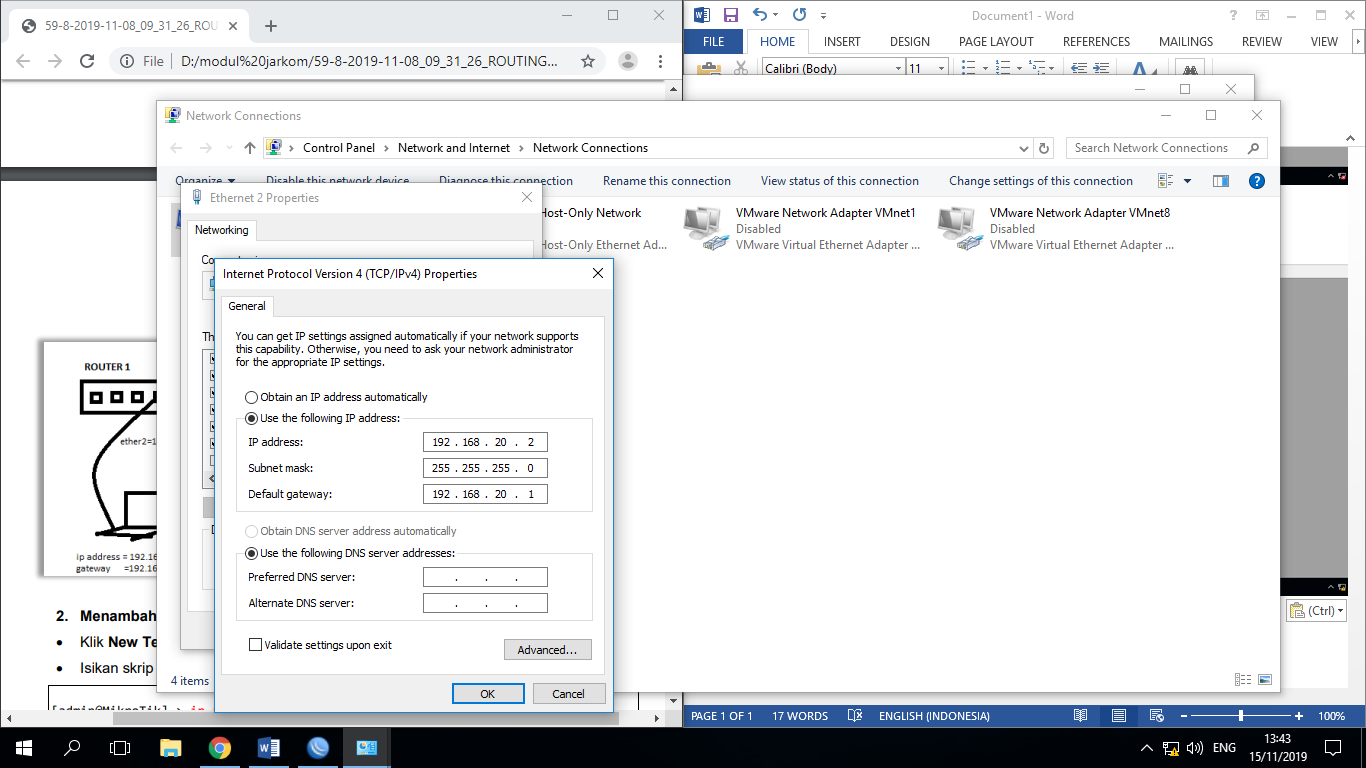
\includegraphics[scale=.4]{Page-5-Image-9}
	\end{center}
	Setting IP  pc di \textit{Control Panel}
	
	\item \textbf{Konfigurasi RIPv2\\}
	\begin{center}
		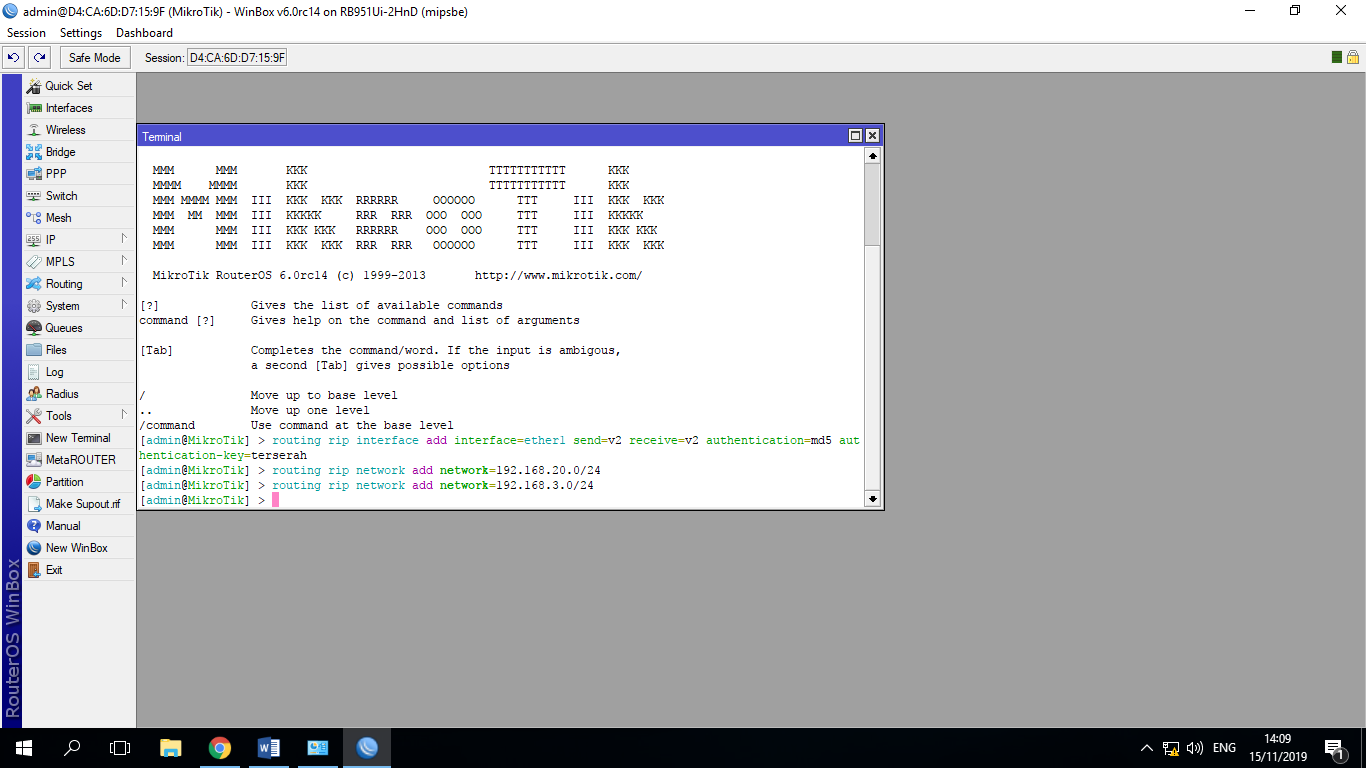
\includegraphics[scale=.38]{Page-6-Image-10}
	\end{center}
	tambahkan RIPv2 menggunakan perintah \\
	\texttt{[admin@MikroTik] > \textcolor{red}{routing rip interface add interface=ether1 send=v2 receive=v2 authentication=md5 authentication=\textit{password} }}\\
	setelah itu masukkan ip dengan perintah\\
	\texttt{[admin@MikroTik] >\textcolor{red}{routing rip network add network=192.168.20.0/24}}\\
	Lalu masukkan IP lagi\\
	\texttt{[admin@MikroTik] >\textcolor{red}{routing rip network add network=192.168.3.0/24}}
	
	\item \textbf{Melihat Hasil Routing}
	\begin{center}
		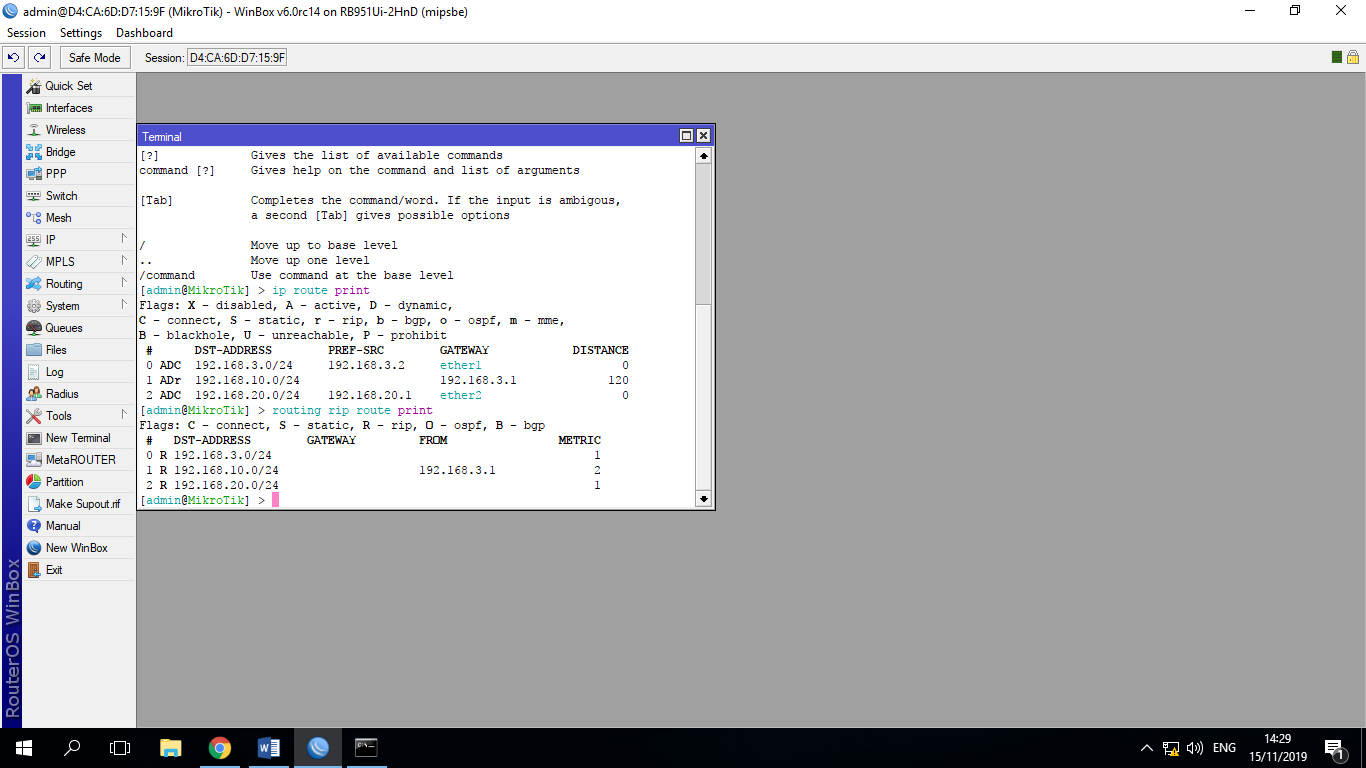
\includegraphics[scale=.4]{Page-6-Image-11}
	\end{center}
	Tampilkan hasil routing dengan perintah\\
	\texttt{[admin@MikroTik] > \textcolor{red}{routing rip route print}}
	
	\newpage
	
	\item \textbf{Menguji Koneksi}
	\begin{center}
		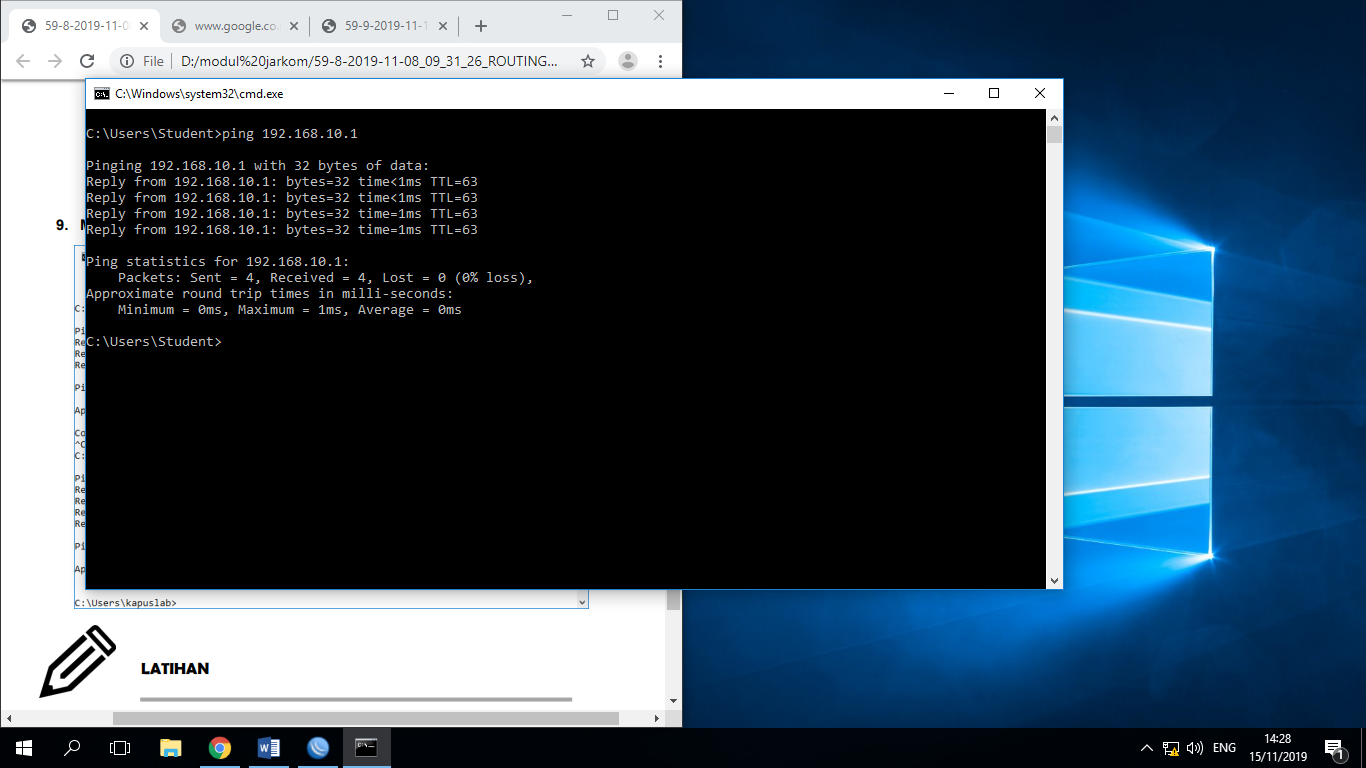
\includegraphics[scale=.4]{Page-7-Image-12}
	\end{center} 
	Uji koneksi dengan ping
	
\end{enumerate}

\newpage

\section{Tugas}
\paragraph{Tabel Routing RIP}
\begin{center}
	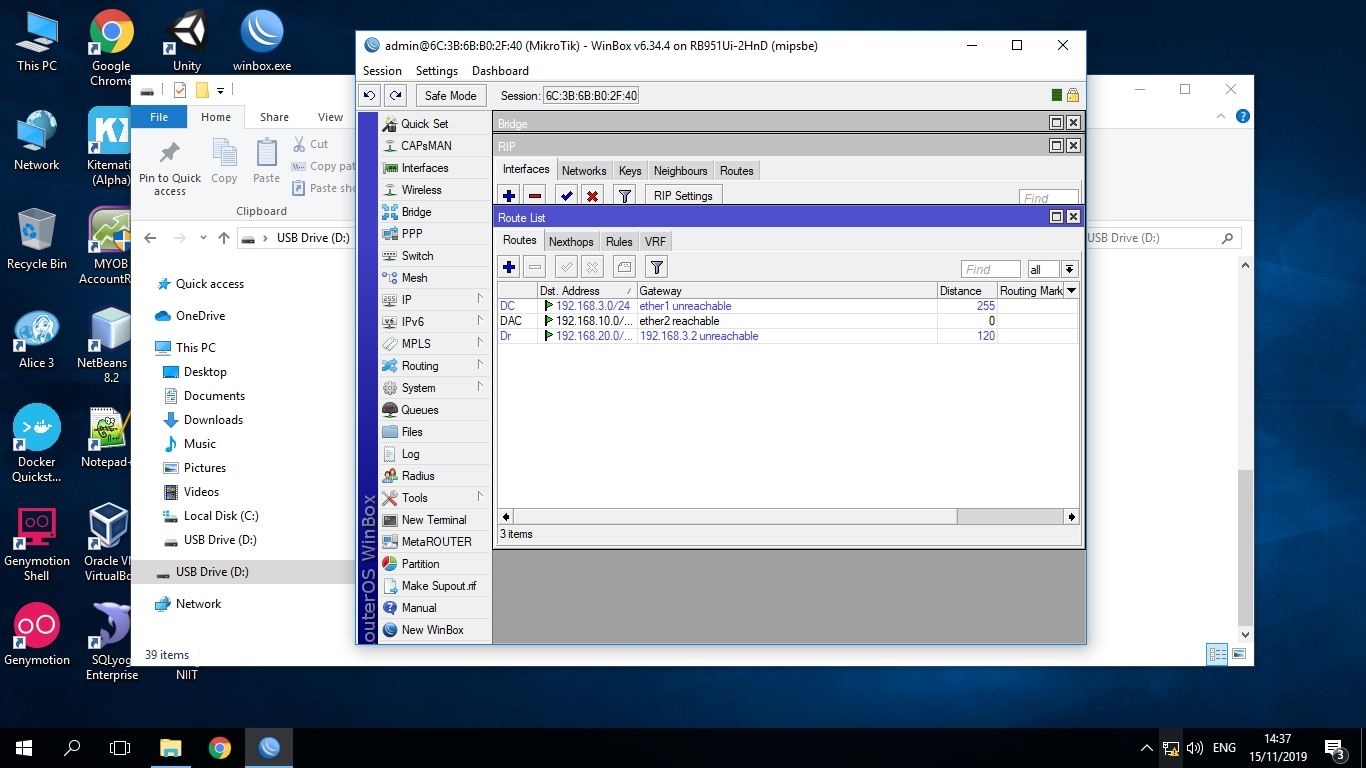
\includegraphics[scale=.4]{image1}
\end{center}
Tabel routing rip berisi daftar IP yang dimasukkan ke routing RIP, dan interfacenya

\newpage

\section{Kesimpulan}
Setelah pertemuan ini mahasiswa mampu menerapkan routing dinamis dengan RIP pada piranti router

\end{document}